Überschüssiges Material wird mit Werkzeugschneiden mechanisch abgetrennt. Dabei entstehen Späne.\\

Die wichtigsten zerspanenden Verfahren sind:
\begin{itemize}
    \item Drehen
    \item Bohren
    \item Fräsen
    \item Schleifen
\end{itemize}

\textbf{Geometrisch bestimmt:} \hfill (Drehen, Bohren, Fräsen)\\
Schneidkeil dringt in Werkstoff ein, elastische und plastische 
Verformung, Fliessen des Werkstoffes, Ausbildung eines Spans, 
Ablaufen des Spans über den Schneidkeil.\\

\textbf{Voraussetzungen:} hohe Härte des Werkzeugs und eine minimale Eindringtiefe.\\
Höhere Produktivität aber auch höhere Ungenauigkeit.\\
Rauheit 3. Ordnung, $R_z > 2.5 \mu m$\\

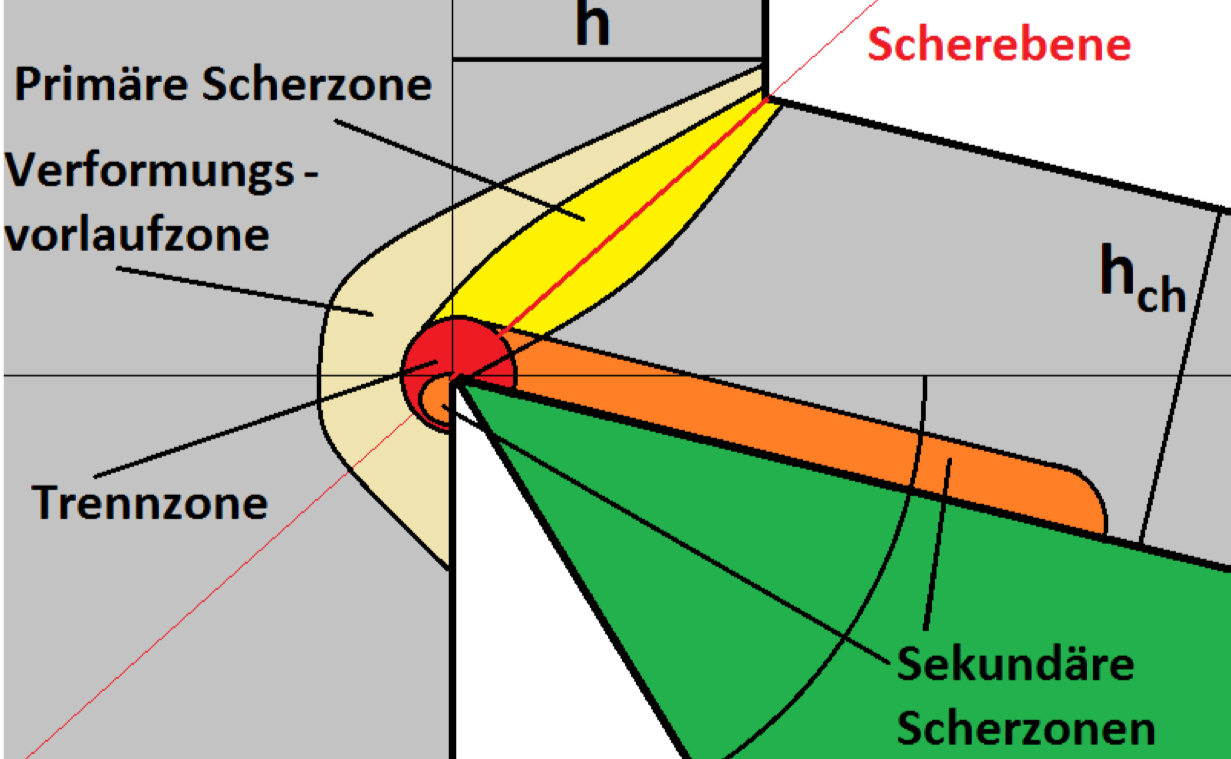
\includegraphics[width=0.8\linewidth]{src/images/Spanen.jpeg}\\
\textbf{Geometrisch Unbestimmt:} \hfill (Schleifen)\\
Abrasivkörner dringen in Wekrstoff ein, elastische und plastische 
Verformung, duktile Werkstoffe fliessen und bilden Mikro-Späne, 
Spröde Werkstoffe bilden Risse und Brechen aus. \\

\textbf{Voraussetzungen:} hohe Härte der Abrasivkörner sowie eine minimale Eindringtiefe.\\
Geringere Produktivität aber mehr Genauigkeit.\\
Eine grosse Porosität gibt Raum für die Späne und dient der Kühlung. \\
Rauheit 5.-6. Ordnung, $R_z < 2.5 \mu m$\\